\documentclass[dvipdfmx]{beamer}
\usepackage{pxjahyper}
%\usepackage[uplatex]{test}
\usetheme[
    block=fill, % ブロックに背景をつける
    progressbar=foot, % 各スライドの下にプログレスバー
    numbering=fraction % 合計ページ数を表示
]{metropolis}           % Use metropolis theme
%\usetheme{CambridgeUS}
\usepackage{float}
\usepackage{booktabs}
\usepackage{ascmac}
\usepackage{fancybox}
\usepackage{amsmath}
\usepackage{mathtools}
\renewcommand{\kanjifamilydefault}{\gtdefault} % 和文デフォルトをゴシック体に
\usepackage{tikz}
\usetikzlibrary {arrows.meta}
\usetikzlibrary {bending}
\usepackage{listings,jvlisting} %日本語のコメントアウトをする場合jvlisting(もしくはjlisting)が必要
%ここからソースコードの表示に関する設定
\lstset{
  basicstyle={\tiny},
  stringstyle={tiny},
  frame={tb},
  breaklines=true,
  columns=[l]{fullflexible},
  numbers=left,
  xrightmargin=0zw,
  xleftmargin=3zw,
  numberstyle={\tiny},
  stepnumber=1,
  numbersep=1zw,
  lineskip=-0.5ex
}

\title{進捗報告}
\date{\today}
\author{水野泰旭}
\institute{弘前大学理工学部電子情報工学科4年}
\subject{}
\begin{document}
  \maketitle

  \begin{frame}{目次}
    \tableofcontents
   \end{frame}

  \begin{frame}
    \section{ハイパーパラメータの調節}
  \end{frame} 
  
  \begin{frame}{学習率による調節}
    \begin{figure}
      \centering
      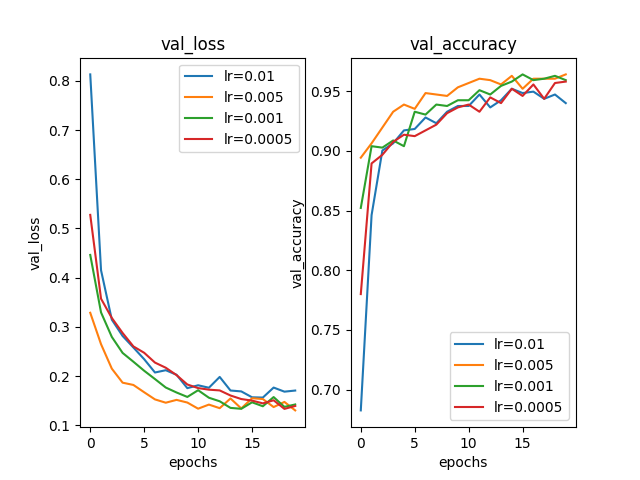
\includegraphics[keepaspectratio, scale=0.6]{images/compare_learning_rate_4v.png}
      \caption{学習率の性能比較}
      \label{fig:compare_lr}
    \end{figure}
  \end{frame}

  \begin{frame}{最適化アルゴリズムによる調節}
    最適化アルゴリズムの種類
    \begin{itemize}
      \item SGD
      \item Adagrad
      \item RMSProp
      \item Adam
    \end{itemize}
  \end{frame}

  \begin{frame}
    \begin{figure}
      \centering
      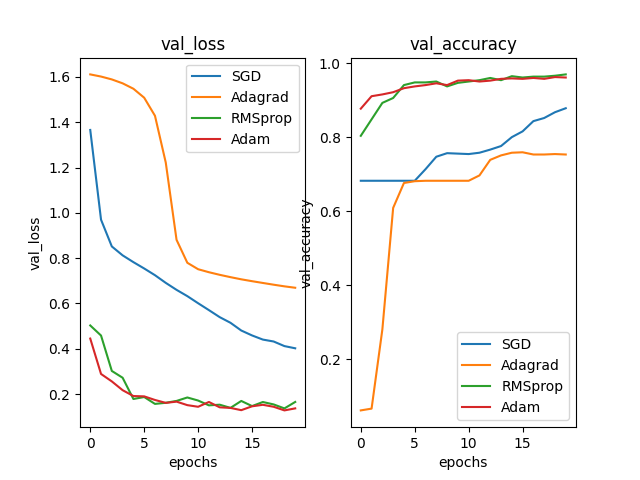
\includegraphics[keepaspectratio, scale=0.6]{images/compare_learning_rate_optimizer.png}
      \caption{最適化アルゴリズムの性能比較}
    \end{figure}
  \end{frame}

  \begin{frame}
    \section{k分割交差検証}
  \end{frame}

  \begin{frame}{手順}
    \begin{enumerate}
      \item 訓練データとテストデータを結合する
      \item データをシャッフルする
      \item 以下の操作をk回繰り返す
      \begin{enumerate}
        \item 訓練データとテストデータに分ける
        \item モデルを作り学習する
      \end{enumerate}
      \item それぞれの学習で得られた正解率の平均を出力する
    \end{enumerate}
  \end{frame}

  \begin{frame}[fragile]{ソースコード}
    \begin{lstlisting}[caption=ksparate\_train.py]
      k = 10
      num_validation = len(images) // k
      for fold in range(k):
          # SEPARATE DATA
          validation_images = images[num_validation * fold: num_validation * (fold + 1)]
          validation_labels = labels[num_validation * fold: num_validation * (fold + 1)]
          train_images = np.concatenate([images[:num_validation * k], images[num_validation * (k + 1):]], axis=0)
          train_labels = np.concatenate([labels[:num_validation * k], labels[num_validation * (k + 1):]], axis=0)
      \end{lstlisting}
  \end{frame}

  \begin{frame}
    \begin{table}[H]
      \centering
      \caption{4分割交差検証の結果}
      \begin{tabular}{cr}
        \hline
        fold & 正解率 \\
        \hline \hline
        0 & 0.991935491561889 \\
        1 & 0.992943525314331 \\
        2 & 0.992439508438110 \\
        3 & 0.993951618671417 \\
        \hline \hline
        平均 & 0.992817535996437 \\
        \hline
      \end{tabular}
    \end{table}
  \end{frame}

  \begin{frame}{まとめ}
    \begin{itemize}
      \item 学習率は0.005とする
      \item 最適化アルゴリズムにAdamを用いる
      \item k分割交差検証の正解率が高いので、原因を調べる
    \end{itemize}
  \end{frame}

\end{document}